\documentclass{article}
\usepackage{graphicx}
\usepackage{enumerate}
\usepackage{setspace}
\usepackage{hyperref}
\usepackage[utf8]{inputenc}
\usepackage[OT1]{fontenc}
\usepackage[french]{babel}
\usepackage{vmargin}
\setpapersize{A4}
\setmargins{15mm}{15mm}{180mm}{260mm}{0pt}{0mm}{0pt}{1.2cm}
\title{Compte rendu OUTILS LIBRES}
\author{REVEL Rémi}
\date{\today}

\begin{document}
\maketitle
\par\noindent\rule{\textwidth}{0.4pt}

\section{\huge{efficatité de l'environnemnt de travail}}
%----------------------------------------Question 1-----------------------------------------------------
\subsection{\large{Desactivation de la souris}}

\subsection*{\normalsize{voici les commande pour desactiver la souris:} } 
\begin{enumerate}
    \item xinput set-prop 4 "Device Enabled" 0

    \item xinput set-prop 6 "Device Enabled" 0

    \item xinput set-prop 7 "Device Enabled" 0
\end{enumerate}

\subsection*{\normalsize{tableau de raccourcis clavier utile:} }    

\begin{center}
   \begin{tabular}{| l | c | }
     \hline
     changer d'application & alt+tab ou windows+tab\\ \hline
     gestionnaire d'application & Touche windows \\ \hline
     Naviguer sur les elements cliquable d'une page web & tab   \\ \hline
     Fermer le navigateur & CTRL+W \\ \hline
     Fermer une appliacation & ALT+F4 \\ \hline
     Changer d'onglet sous Brave & CTRL+1,2,3,...   \\ \hline
     Ouvrir un nouvelle onglet & CMD+T \\ \hline
     faire une recherche & F6 \\ \hline
   \end{tabular}
 \end{center}
 
 %---------------------------------------------------------------------------------------------
 
 %----------------------------------------question 2-----------------------------------------------------
 
 \subsection{\large{S'ameliorer a la dactylographie}}
 le site que j'ai retenu pour s'ameliorer en dactylographie est \href{https://10fastfingers.com/typing-test/french}{10fastfingers}. \par On peut s'entrainer sur des mots aleatoire, ou sur nos propres texte, le site est disponible dans plusieurs langue.

\begin{center}
    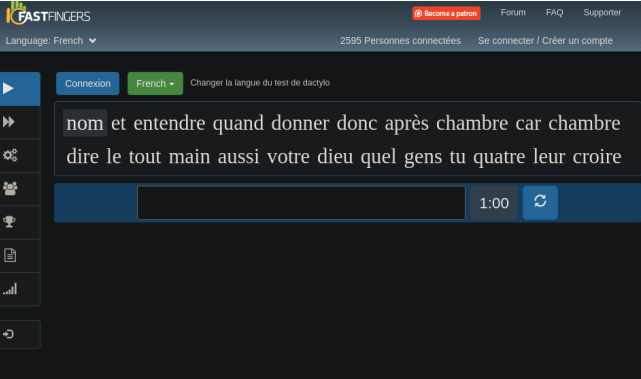
\includegraphics[scale=0.7]{Images/fastfinger.png}
\end{center}

%---------------------------------------------------------------------------------------------

%---------------------------------------------Question 3------------------------------------------------

\subsection{\large{Tutoriel pour VIM}}

\begin{center}
   \begin{tabular}{| l | c | }
     \hline
     insertion & i\\ \hline
     enregister & :w\\ \hline
     quitter & :q \\ \hline
     aller au debut du fichier & :1 \\ \hline
     aller a la fin du fichier & :\textdollar \\ \hline
     annuler une action & u \\ \hline
     recherche d'une occurence & /occurence \\ \hline
     activer coloration syntaxique & :syntax on \\ \hline
     templacer du texte & :s/origin/replacement/g \\ \hline
   \end{tabular}
 \end{center}
 
 pour definir VIM comme editeur par defaut on a juste a rentrer cette commande: \par update-alternatives --set editor /bin/vim
 
 %---------------------------------------------------------------------------------------------
 
 %---------------------------------------------Question 4------------------------------------------------
 
 \subsection{\large{Bash history}}
 
 Mon mot de passe n'apparait pas dans le bash history, donc il n'y a pas d'informations sensible.\par
 Les historiques sont propres a chaque shell utilisé. \\
 
 Pour eviter de poluer notre historique avec des commande basique on peut les exclures avec cette commande : \par
 export HISTIGNORE="ls : cd : pwd"
 
  %---------------------------------------------------------------------------------------------
  
  %---------------------------------------------Question 5------------------------------------------------
  
  \subsection{\large{Alias de fonction}}
  Les commandes presentes ci dessous sont a placer dans le .bashrc
  
  \begin{center}
        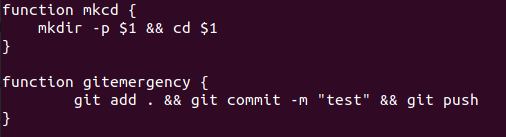
\includegraphics[scale=0.7]{Images/function.png}
  \end{center}
    
 %---------------------------------------------------------------------------------------------
 
 %---------------------------------------------Question 6------------------------------------------------
 
 \subsection{\large{Script}}
 Ce script est fait pour la sauvegarde des données des utilisateurs de la machine.
 
 \begin{center}
        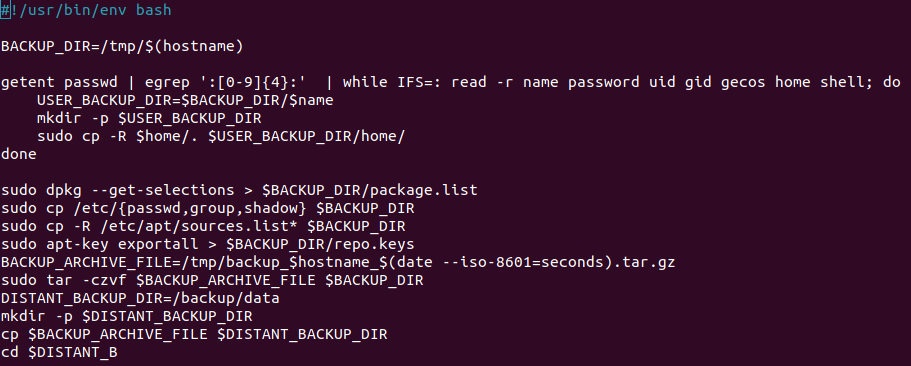
\includegraphics[scale=0.5]{Images/save.png}
 \end{center}
    
 %---------------------------------------------------------------------------------------------
 
 \newpage
 
 %---------------------------------------------Question 7------------------------------------------------
 
 \subsection{\large{customisation avec OH MY ZSH}}
 Dans le fichier du theme oh y zsh que l'on a selectioné on y rajoute ceci pour pouvoir voir le status de nos Vagrant et notre statut git.
 
 \begin{center}
        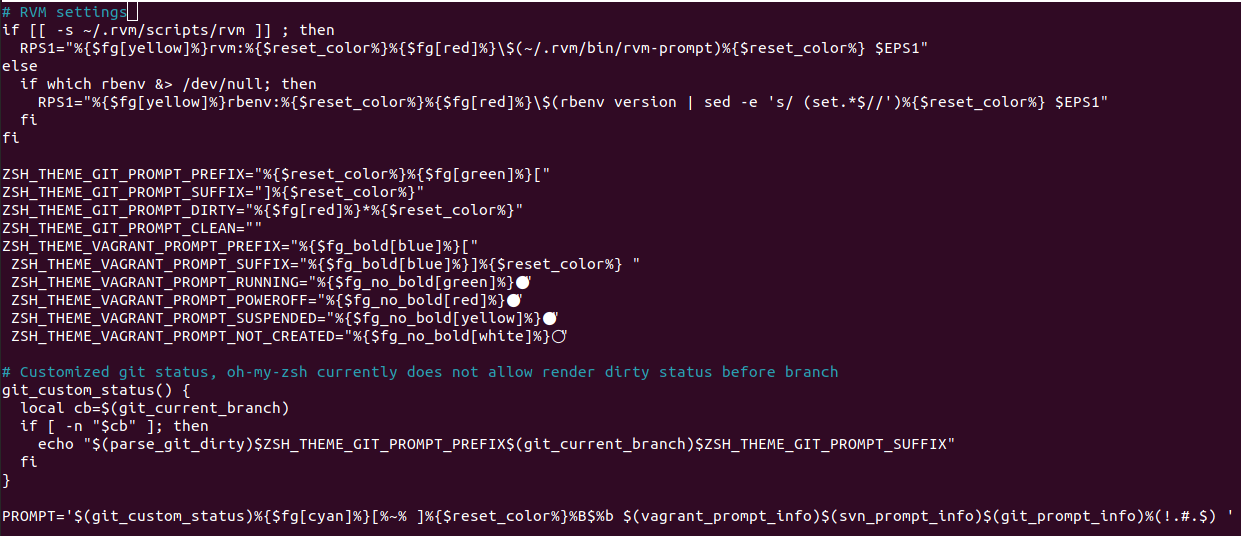
\includegraphics[scale=0.43]{Images/theme.png}
 \end{center}
    
 %---------------------------------------------------------------------------------------------
 
 %---------------------------------------------Question 8------------------------------------------------
 
  \subsection{\large{Raccourci clavier}}
  
  Pour faire un raccourcis clavier qui start ou stop apache en faisant CTRL+A, on place ce petit bout de code dans notre .bashrc
  
  \begin{center}
        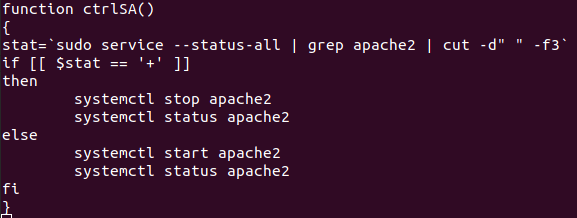
\includegraphics[scale=0.6]{Images/CTRLA.png}
  \end{center}
  
 %---------------------------------------------------------------------------------------------
 
  \newpage
  
 %---------------------------------------------Question 9------------------------------------------------
 
 \subsection{\large{Emulateur de terminaux}}
 
 \subsection*{\normalsize{Sakura :} } 
 C'est un terminal assez simple, il est leger, il fait rien de plus que le terminal qui est present de base sur debian, son avantage un noir profond ce qui fait bien ressortir les couleurs, on a la possibilité d'avoir plusieurs onglets. Couplé au shell fish qui possedent un coloration syntaxique et de l'auto completion basé sur l'historique, ca rend le terminal interessant.
 
 \begin{center}
        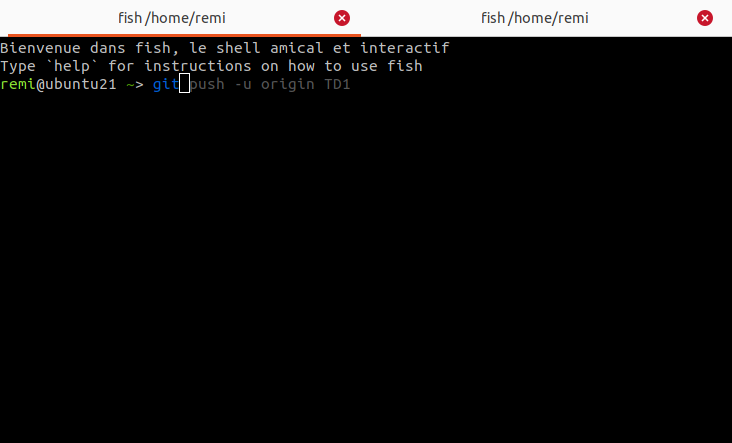
\includegraphics[scale=0.5]{Images/sakura.png}
 \end{center}
 
 \subsection*{\normalsize{urxvt :} } 
 C'est un terminal tres leger, il prend tres peu de ressource, il n'y a pas de possibilité de faire un nouvel onglet. Il est pas tres jolie a voir
 
 \begin{center}
        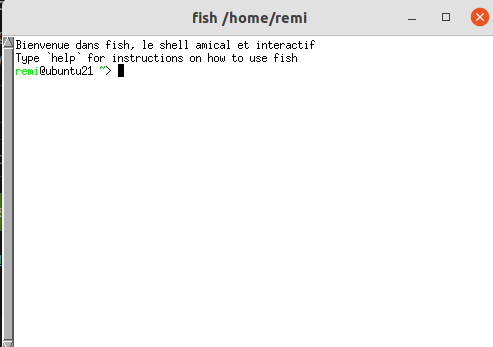
\includegraphics[scale=0.6]{Images/urxvt.png}
 \end{center}
 
 \newpage
  
 \subsection*{\normalsize{Tilix :} } 
C'est un terminal beaucoup plus avancé que les autres, on peut le customiser comme on veut, on peut aussi modifier les raccourcis clavier. Les fenetres de ce terminal peuvent etre logé sous forme de mosaique. Il y a la possibilité que les commandes que l'on tape soit répliqué sur d'autres terminaux. Pour un admin sys, c'est un tres bon terminal.
 
 \begin{center}
        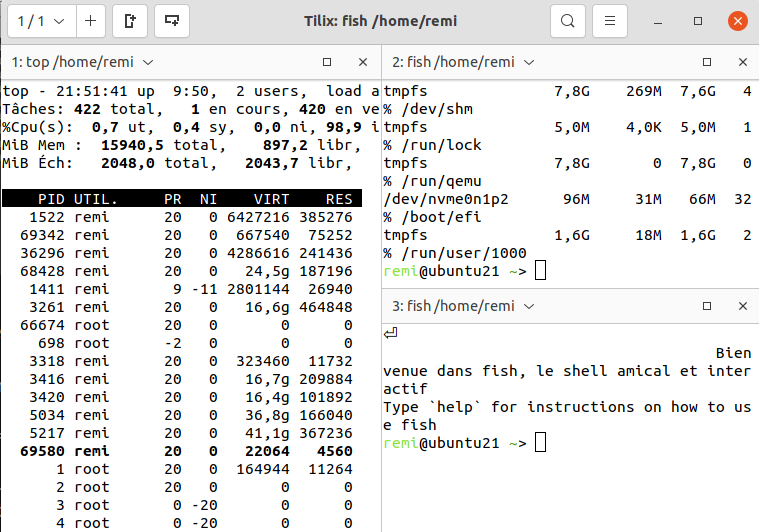
\includegraphics[scale=0.6]{Images/tilix.png}
 \end{center}
 
 %----------------------------------------FIN TD1------------------------------------------
 
 
\end{document}
